\documentclass[conference]{IEEEtran}
\usepackage{amsmath,amssymb,graphicx,booktabs,array}
\usepackage[hidelinks]{hyperref}
\usepackage{url}
\usepackage{balance}
\providecommand{\StudentID}{}
\newcommand{\code}[1]{\texttt{#1}}
\newcommand{\Qthree}{Qwen3-4B}
\newcommand{\Qtwo}{Qwen2.5-7B}
\graphicspath{{./}{../manuscript/}}
\title{Auditing Peer-Signal Sensitivity in Campus LLM Agents}
\author{\IEEEauthorblockN{Wenkang Zhu}\IEEEauthorblockA{DASE7506 Advanced Machine Learning Methods\\The University of Hong Kong\ifx\StudentID\empty\else\\\StudentID\fi}}
\begin{document}
\maketitle
\pagestyle{plain}
\begin{abstract}
Does a campus language-model agent choose to study more often when its prompt reports stronger recent peer study? We audit an inherited single-step interface using four fixed profiles, three peer levels, and energy and satiety controls. A frozen protocol produced 2,040 completions across Qwen3-4B-Instruct-2507, Qwen2.5-7B-Instruct, and a Qwen3 afternoon context; 1,999 passed its parser, with no truncations. At 11:00, one Qwen3 profile increased valid-study responses from 1/30 to 9/30; the other three produced none. All 12 conservative simultaneous peer intervals include zero, leaving family-wide evidence inconclusive. A post-result measurement audit finds that 37 of 41 rejected outputs contain legal exercise decisions but exceed the parser's hard duration bound, although the prompt describes that bound as suggested. Action-only extraction explains these outputs without changing any study count or target-action contrast. We contribute complete dose curves, uncertainty and batch sensitivity analyses, and a reproducible separation of decision outcomes from interface compatibility. These results concern prompt-conditioned decisions rather than human peer influence. Code, data, and reproduction instructions: \url{https://github.com/zwkcyy/dase7506-mp3/tree/main/campus-peer-audit}.
\end{abstract}
\begin{IEEEkeywords}
LLM agents, controlled evaluation, social simulation, uncertainty, reproducibility
\end{IEEEkeywords}

\section{Introduction}
Our research problem is whether increasing a numerical summary of peers' recent study changes a campus LLM agent's probability of returning a valid study decision, and whether the observed response persists across profiles, checkpoints, and a second decision time. A simulator can produce plausible activity narratives without reliably responding to its intended inputs. Measuring an individual decision component is therefore useful before interpreting population trajectories or social feedback.

The supplied course-project archive contains an Agent-Kernel campus adaptation, profile descriptions, a decision-prompt builder, and earlier peer-probe ideas. We inherit these components and turn the probe into a controlled, fully accounted experiment. Our contributions are (i) a frozen 2,040-completion evaluation spanning two checkpoints and a time extension, with complete three-level peer responses; (ii) uncertainty analysis that distinguishes a local pointwise finding from a family-wide claim; and (iii) a measurement audit showing how an auxiliary parser rule can hide an otherwise readable action. The public release retains every formal reply and supports CPU reproduction of the reported results.

The scope is deliberately narrow. Each completion is a fresh decision with no evolving memory or reciprocal interaction. Thirty completions of one prompt are Monte Carlo observations of a model, not thirty students. The primary outcome is the probability of obtaining a valid \code{study} decision per completed call. We also retain invalid outputs, conditional-on-valid rates, and every alternative action.

Three questions organize the study: (1) does the peer-summary field change this outcome for each fixed profile; (2) how do the observed responses compare between two checkpoints and between 11:00 and 16:00 for Qwen3; and (3) do basic-state controls elicit their intended target actions? The second question is partly descriptive: checkpoint family, training, and size differ together, and the time extension covers only Qwen3.

A fourth, explicitly post-result question concerns measurement: do parser rejections indicate unreadable actions, or incompatibility in auxiliary fields? This distinction matters because a validity-aware outcome combines action selection with interface acceptance.

\section{Related Work}
Generative Agents evaluates a 25-agent environment with memory, reflection, and planning \cite{park2023generative}; Agent-Kernel provides the framework provenance for the supplied implementation \cite{mao2025agentkernel}. Our single-step experiment omits these system dynamics, so it cannot reproduce their system-level evaluations. This distinction makes the experiment auditable but limits its conclusions.

RoleLLM introduces RoleBench for evaluating and improving character role-playing \cite{wang2024rolellm}. SOTOPIA evaluates agents through interactive social scenarios and goal-oriented behavior \cite{zhou2024sotopia}. Our task instead measures controlled input sensitivity and the effect of output-processing rules within one inherited interface. We have no optimal-action or human labels, so study frequency is an outcome, not accuracy or a benchmark score.

Persona conditioning has also been studied as a way to construct synthetic human responses. Argyle et al. compare demographic conditioning with survey data \cite{argyle2023out}, and Aher et al. examine replication of human-subject findings \cite{aher2023using}. These studies use external targets that our campus task lacks. Santurkar et al. document opinion-distribution mismatches despite group steering \cite{santurkar2023whose}; Bisbee et al. show that apparently plausible synthetic averages can conceal problems in variation and associations \cite{bisbee2024synthetic}. These findings motivate task-specific validation, rather than establishing the errors of the present checkpoints. Here, a profile-dependent output is evidence about a prompt, not demographic fidelity or human behavioral realism.

\section{Controlled Decision Protocol}
\subsection{Interface and fixed context}
The inherited Chinese interface requests one of seven actions: \code{study}, \code{go\_class}, \code{exercise}, \code{chat}, \code{rest}, \code{eat}, or \code{wander}. The system prompt requests JSON and permits optional duration and contextual-effect fields. It describes a duration of 1--6 ticks as suggested; the frozen evaluator nevertheless enforces that range whenever duration is supplied. The user prompt contains behavioral principles, state values, action examples, and peer information. Its instruction to prioritize basic needs and fit identity and goals is retained; successful state responses can therefore reflect instruction following.

All main conditions describe 11:00 on a sunny weekday in a dormitory, with no class duty, empty recent-action and memory text, and three peers currently resting. Their actions and locations never change. The peer intervention changes only the displayed scalar summarizing \emph{recent} peer study intensity; it does not create studying peers or a live social network.

The four existing profile bundles P01--P04 vary identity, personality description, habits, and goals together. Names are replaced by the same anonymous label. Numerical conscientiousness is fixed at 0.65 and motivation at 0.50, with course group A1. Thus, profile comparisons concern complete text bundles, not isolated psychological traits. Brief translations appear in Appendix A; the repository preserves the exact Chinese inputs.

\subsection{Levels and factorial layout}
The manipulation range is calibrated using 458 student LLM-decision records with successful parsing from one supplied historical simulator trace. The filter retains class-duty records, including 99 such decisions. These rows define an interface operating range, not independent students, human ground truth, or evaluation outcomes. Their original serving checkpoint is not established. Quantiles use linear interpolation at position $(n-1)p$; the prompt builder then rounds values to two decimal places.

\begin{table}[t]
\caption{Values actually displayed in the prompt. Unchanged factors remain at their middle values.}
\label{tab:levels}
\centering\small\setlength{\tabcolsep}{3.5pt}
\begin{tabular}{lccc}\toprule
Field & Low (q10) & Middle (q50) & High (q90)\\\midrule
Recent peer study & 0.06 & 0.13 & 0.24\\
Energy & 0.33 & 0.50 & 0.81\\
Satiety & 0.46 & 0.70 & 0.95\\
Social state & -- & 0.98 & --\\
Mood & -- & 0.98 & --\\\bottomrule
\end{tabular}
\end{table}

The main design has 28 cells: four profiles crossed with three peer levels (12 cells), low/high energy (eight), and low/high satiety (eight). Each cell receives 30 calls, totaling 840 per checkpoint. State arms hold the peer summary at 0.13 and vary only their own field. The center peer cell is not sampled again for the state arms. The source variable named \code{hunger} is displayed as \emph{satiety}: lower values mean less satisfied. The intended controls are more \code{rest} at low energy and more \code{eat} at low satiety.

Offline checks confirm a common system prompt, anonymous names, distinct rounded levels, unique inputs, and one changed user-prompt line per within-profile intervention relative to its center. These checks exclude unintended text changes within an arm; they do not establish that independently chosen marginal quantiles form a common real-world situation.

\subsection{Pre-result freezes and actual execution}
Before formal sampling, the scientific plan fixed both 840-call checkpoint runs and a 360-call, peer-only Qwen3 extension at 16:00. The latter repeats the 12 peer cells without state controls. Scientific and execution manifests record the chronology. A separate 112-call set of interface and capacity pilots was excluded from every formal result. Execution choices were finalized before formal sampling, and no failures were selectively replaced.

We used Qwen3-4B-Instruct-2507, a non-thinking-only checkpoint \cite{qwen3card}, and Qwen2.5-7B-Instruct \cite{qwen25card}. Immutable revisions are listed in Appendix B. The actual engine was direct, in-process Transformers 4.57.1, with PyTorch 2.8.0+cu128, BF16, SDPA attention, and batch size 16 on one RTX 4090. This replaces the earlier pilot HTTP adapter; formal data contain no HTTP requests. Every conversation starts fresh. Within each run, a fixed shuffled schedule interleaves cells, with base seed 20261122 plus the one-based batch index. Rows share a batch PRNG stream; they are not independently reseeded simulation episodes.

Sampling is explicit: temperature 1, top-$p$ 1, top-$k$ 0, repetition penalty 1, maximum 1,024 new tokens, and \code{use\_model\_defaults=False}. Checkpoint generation defaults therefore do not silently determine the experiment. Left-padded token inputs, masks, unpadded token lists, effective configuration, model identity, raw content, output tokens, and finish reasons are logged. The inherited literal suffix \code{/no\_think} is fixed across conditions; it is not an experimental reasoning-mode comparison. Source, input, and output hashes support internal consistency checks, not cryptographic attestation or independent reproduction of a stochastic completion.

\section{Outcomes and Strengthened Analysis}
\subsection{Frozen accounting and contrasts}
An output is valid if the pre-result frozen parser finds a decision object with a legal action, the checked optional fields have acceptable types/ranges, and termination is EOS/stop rather than length exhaustion. Optional \code{duration\_ticks}, if present, must be an integer from 1 to 6; \code{contextual\_effects}, if present, must be an object. We retain this original definition throughout the primary analysis. It measures compatibility with the evaluator, not semantic correctness, strict adherence to every prompt instruction, or validity of every nested effect.

For cell $c$, let $N_c$ be completed calls, $V_c$ valid outputs, and $K_{c,a}$ valid outputs choosing action $a$. We report
\begin{equation}
\widehat\theta_{c,a}=K_{c,a}/N_c,\qquad
\widehat p_{c,a}=K_{c,a}/V_c.
\end{equation}
The first is the joint valid-and-action probability; the second is conditional on validity. Invalid text is not treated as an observed alternative action. Uncompleted calls would not be imputed as failures; in the present data all planned calls completed. The primary contrast is high-minus-low peer signal for \code{study}; state contrasts are low-minus-high for their target action. \code{go\_class} is always separate.

The frozen analysis uses Wilson 95\% intervals for proportions and Newcombe's independent-proportion Wilson hybrid intervals for differences \cite{newcombe1998}. These are pointwise intervals, not simultaneous bands. For invalid-output sensitivity we retain the assignment range
\begin{equation}
\left[K_{c,a}/N_c,\;(K_{c,a}+N_c-V_c)/N_c\right].
\end{equation}
It is a worst-case accounting range, not a confidence interval or proof that an invalid response has a latent true action.

\subsection{Post-result improvements}
After inspecting the original results, we fixed a separate enhancement plan on 23 November 2026. It adds no model calls and leaves the original freezes, outputs, and analyses unchanged. These improvements must not be represented as pre-result registration.

First, we include \emph{all} 12 profile-specific peer contrasts across the three runs in one family. Clopper--Pearson endpoint intervals \cite{clopper1934} receive two-sided error $0.05/24$ for its 24 endpoint proportions. If endpoint intervals are $[L_A,U_A]$ and $[L_B,U_B]$, a difference interval is
\begin{equation}
[L_A-U_B,\;U_A-L_B].
\end{equation}
The union bound gives at least 95\% simultaneous coverage for this family under binomial marginal assumptions. The 16 state contrasts form a separate family with 32 endpoints and error $0.05/32$ per endpoint. The two families together are not claimed to have 95\% joint coverage. Their additional width reflects exact marginal intervals, rectangular difference bounds, and multiplicity protection together; it is not solely a multiple-comparison penalty. We also form a sensitivity envelope allowing invalid counts to be assigned to the target.

Second, we resample observed computational batches with replacement 10,000 times within each run, retaining all rows of each selected batch, using separately fixed seeds. Percentile intervals are a check on computational grouping, not evidence that batches are random population clusters. Shared PRNG alone does not establish dependence, and the original binomial assumptions are not thereby proven. Undefined resamples are counted rather than replaced by zeros. A bootstrap cannot create unseen successes in an all-zero cell, so its zero-width interval at a floor is not evidence of certainty; the exact binomial intervals remain necessary.

Third, we display all seven valid actions plus invalid outputs. Model and time differences of peer contrasts are explicitly exploratory, with no claim of a fully crossed model-by-time design. No p-values, post-hoc action merging, or favorable-cell resampling are used.

\subsection{Post-result measurement audit}
On 24 November, after observing the rejection categories, we specified an additional CPU-only audit. An independently implemented parser compares the frozen rule with \emph{action-only extraction}: termination must still be EOS/stop, the same first-to-last-brace substring must parse as a JSON object, and its action must be one of the seven legal labels. Only the auxiliary duration/contextual-effect checks are relaxed. We neither repair malformed JSON nor map near-matching actions to legal ones. A separate implementation verifies the resulting census and contrasts.

This diagnostic does not replace the primary outcome. It identifies which rejected outputs already contain an interpretable action, and recomputes all cell counts and all 28 target contrasts under both rules. Agreement of study numerators would establish robustness to this specific processing choice; it would not establish robustness to arbitrary repairs, new prompts, or simulator execution requirements.

\section{Results}
\subsection{Complete execution and validity}
\begin{table}[t]
\caption{Formal completion accounting. Every run had zero truncated outputs; pilots are excluded.}
\label{tab:completion}
\centering\small
\begin{tabular}{lrrr}\toprule
Checkpoint/context & Calls & Valid & Invalid\\\midrule
\Qthree{}, 11:00 & 840 & 821 & 19\\
\Qthree{}, 16:00 & 360 & 342 & 18\\
\Qtwo{}, 11:00 & 840 & 836 & 4\\\midrule
Total & 2,040 & 1,999 & 41\\\bottomrule
\end{tabular}
\end{table}
All 2,040 scheduled calls completed (Table~\ref{tab:completion}). Frozen-parser acceptance was 97.7\%, 95.0\%, and 99.5\% in the three runs, respectively. No completion reached the token limit. Independent CPU checks verified complete per-cell quotas, model revisions, frozen source/configuration hashes, seeds, token/content records, parser decisions, and analysis counts. They verify artifact consistency without rerunning a model.

\subsection{Peer responses and multiplicity}
At 11:00, Qwen3 P02 produced valid \code{study} counts of 1, 6, and 9 out of 30 at the three peer levels (Fig.~\ref{fig:dose}). Its high-minus-low contrast is +26.7 percentage points (pp), with pointwise 95\% interval [7.8, 44.8] pp. All 90 outputs for this profile's peer arm are valid, so validity conditioning does not change this estimate. P01, P03, and P04 produced zero valid-study responses at every peer level. P03 had nine rejected peer-arm outputs, whose readable actions are examined below.

Qwen2.5's low/middle/high study counts were 10/8/12 for P01, 25/24/28 for P02, 3/1/0 for P03, and 2/2/4 for P04, each from 30 calls. Corresponding high-minus-low differences are +6.7, +10.0, -10.0, and +6.7 pp. A monotone dose pattern is therefore not shared across profiles. At the low peer level, Qwen2.5 P02 already studies in 25/30 calls, leaving only 16.7 pp of positive headroom compared with 96.7 pp for Qwen3 P02. Comparing their raw differences alone can conflate responsiveness with baseline policy.

The exploratory P02 difference of peer contrasts (Qwen2.5 minus Qwen3) is -16.7 pp, with batch-resampling sensitivity interval [-39.3, +5.0] pp. Thus, a positive pointwise interval for one checkpoint and an interval including zero for the other do not establish that their peer responses differ. These cross-run intervals are post-result diagnostics under the qualifications in Section VI.

\begin{figure*}[t]
\centering
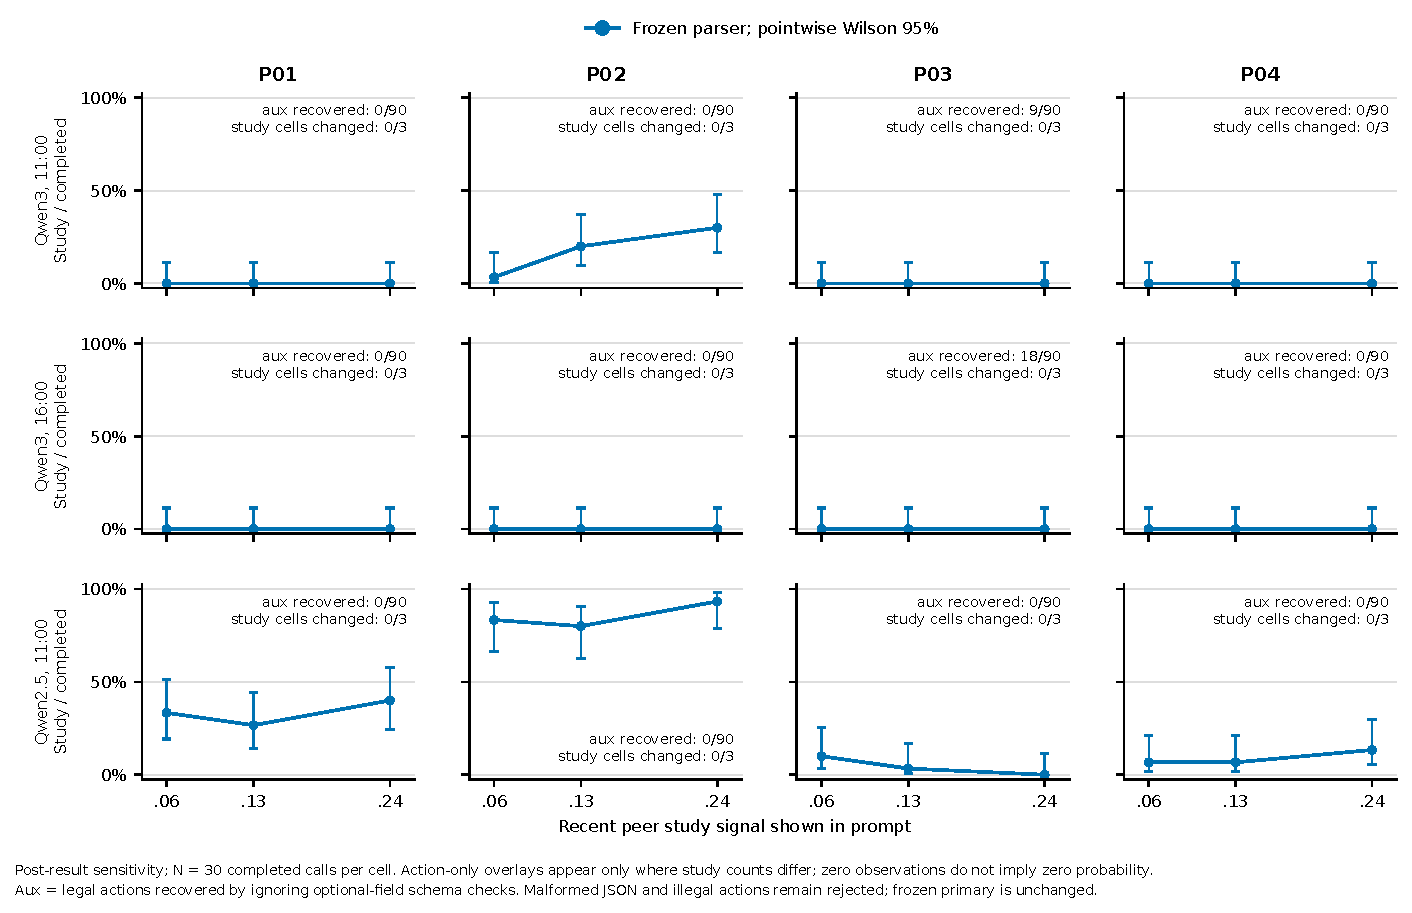
\includegraphics[width=\textwidth]{figures/peer_dose_curves.pdf}
\caption{Complete peer-dose study responses, including all four profiles and three runs. Each point uses 30 completed calls; bars are pointwise Wilson 95\% intervals, not simultaneous bands. Lines connect the three displayed values for readability and do not fit a continuous dose-response function. Action-only extraction leaves every study numerator unchanged.}
\label{fig:dose}
\end{figure*}

% Generated by tools/build_paper_tables.py from robustness.json.
The strengthened family-wide intervals change the interpretation of the local result (Fig.~\ref{fig:overview}A). All 12 peer intervals include zero. For Qwen3 P02 at 11:00, the simultaneous interval is [-17.7, 59.5] pp, substantially wider than its pointwise interval. This conservative result does not prove no effect; it shows that the present data and family-wide criterion do not support a positive conclusion selected from all 12 contrasts.

Batch resampling gives a pointwise interval of [11.1, 43.9] pp for the same profile. It retains a positive local response under this grouping sensitivity, while neither addressing multiplicity nor expanding the target to human students. All 10,000 resamples for every contrast were defined. At zero-success boundaries several bootstrap intervals collapse to [0, 0]; these are empirical-support artifacts, not substitutes for binomial uncertainty.

\begin{figure*}[t]
\centering
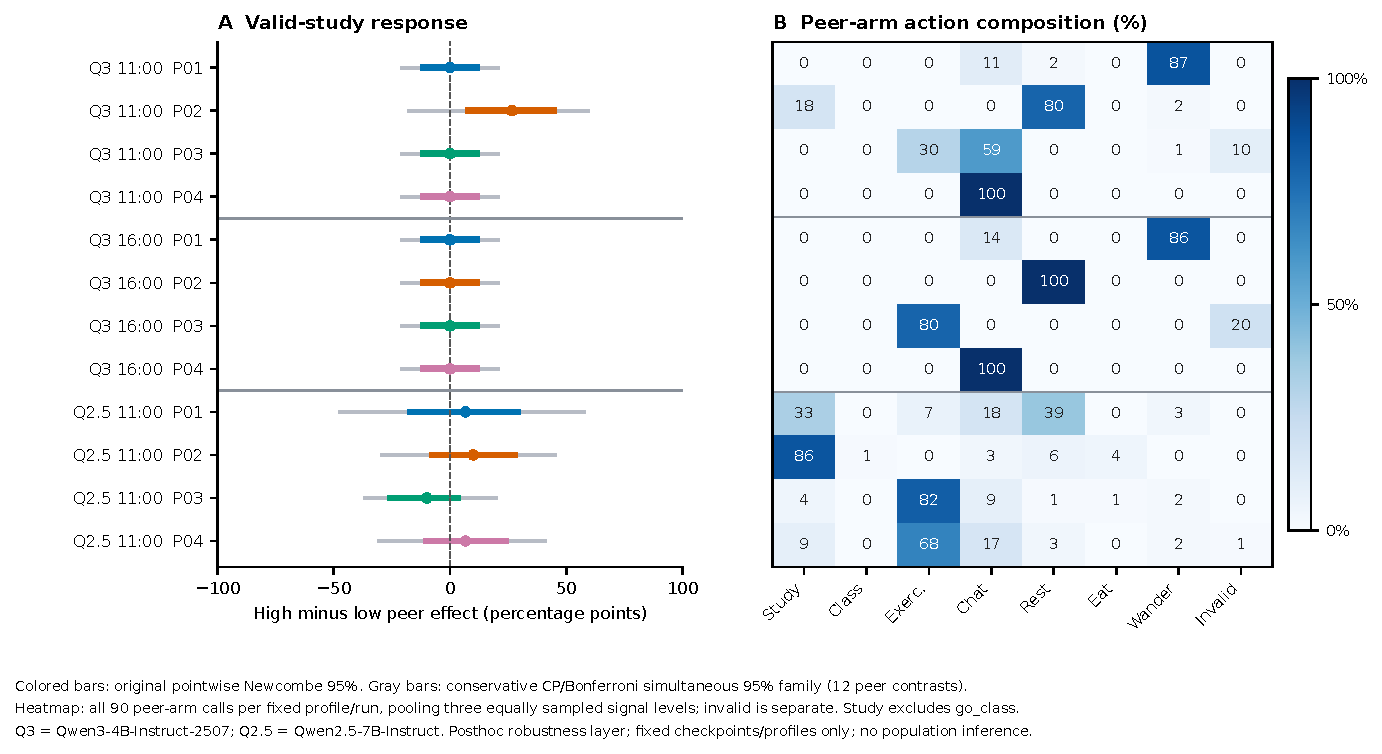
\includegraphics[width=\textwidth]{figures/robustness_overview.pdf}
\caption{Peer-response audit. (A) High-minus-low valid-study differences: colored bars are original pointwise Newcombe 95\% intervals; gray bars are conservative Clopper--Pearson/Bonferroni intervals with at least 95\% simultaneous coverage for the complete 12-contrast peer family under the stated assumptions. (B) Seven valid actions plus invalid outputs, pooling the three equally sampled peer levels (90 completed calls per profile/run). Pooling describes baseline composition; it is not the peer-effect estimator. Q3 and Q2.5 denote the two fixed checkpoints.}
\label{fig:overview}
\end{figure*}


\subsection{Time context, actions, and validity sensitivity}
At 16:00, all 12 Qwen3 cells had zero valid-study outputs. P03 accounts for all 18 parser rejections in that run; its low/high endpoints have 8/4 rejections. Before reading the rejected actions, the mechanical invalid-assignment range for this study contrast is [-26.7, +13.3] pp. The measurement audit below narrows the interpretation by identifying all 18 actions as exercise. Zero study successes with 30 calls still has a pointwise Wilson upper bound of approximately 11.4\%; it does not imply that the underlying probability is exactly zero.

Figure~\ref{fig:overview}B shows why study alone cannot characterize the complete policy: a study floor can coexist with allocation among other actions. The Qwen3 P02 afternoon-minus-morning peer contrast is -26.7 pp, with exploratory batch interval [-43.9, -11.1] pp. Time comparisons concern only this checkpoint and two fixed contexts. They do not constitute an independent replication or a general time effect, and the interval inherits the cross-run limitations below.

The observed state responses are concentrated in a subset of conditions. For Qwen3 P02, low-minus-high energy increases valid \code{rest} by 56.7 pp (pointwise interval [35.8, 72.6] pp). Its simultaneous control-family interval is [6.4, 82.7] pp: it is the only one of the 16 controls excluding zero. For Qwen2.5 P02 the corresponding increase is 23.3 pp (pointwise [5.1, 41.3] pp), but its simultaneous interval is [-20.6, 56.9] pp. Low-satiety \code{eat} differences are zero for all Qwen3 profiles and range from -3.3 to +6.7 pp for Qwen2.5. These data neither establish uniform sensitivity nor rule out smaller target responses. The fixed state levels, other high state values, and inherited examples constrain what these controls test. Table~\ref{tab:allcontrols} reports every state contrast.

\subsection{Separating actions from parser compatibility}
% Generated from measurement_audit/audit.json; frozen primary retained.
\begin{table}[t]
\caption{Frozen parser versus action-only extraction. Action-only retains EOS, parseable JSON, and a legal action; auxiliary-field checks alone are relaxed. Counts cover all arms.}
\label{tab:measurement}
\centering\small\setlength{\tabcolsep}{3pt}
\begin{tabular}{lrrrr}\toprule
Run & Calls & Frozen & Action-only & Added\\\midrule
Q3 11:00 & 840 & 821 & 840 & 19\\
Q3 16:00 & 360 & 342 & 360 & 18\\
Q2.5 11:00 & 840 & 836 & 836 & 0\\
\midrule
Total & 2,040 & 1,999 & 2,036 & 37\\
\bottomrule\end{tabular}
\end{table}


All 37 additionally readable decisions choose \code{exercise} and belong to P03: 19 at 11:00 and 18 at 16:00. Of these, 36 use \code{duration\_ticks}=300 and one uses 360. The numbers show incompatibility with the evaluator's 1--6 bound; their intended units cannot be established from this audit. Since the prompt only suggests that bound, calling every rejection a failure to choose an action would overstate what failed.

Action-only extraction changes no study numerator in any of the 68 cells, and none of the 12 peer or 16 state target-action contrasts. It does change conditional-on-accepted denominators for P03, as well as its exercise accounting. Thus, the primary study findings survive this specific relaxation while apparent Qwen3 action unreadability disappears. The four remaining Qwen2.5 outputs comprise two malformed JSON replies and two illegal action labels; we leave all four unresolved. Neither JSON repair nor interpreting \code{studying} as \code{study} is permitted.

\section{Discussion and Limitations}
Two findings guide interpretation. First, a local pointwise peer estimate remains inconclusive under the complete simultaneous family; broad intervals establish neither absence nor equivalence. Second, 37 of 41 parser rejections arise in an auxiliary duration field, although all 37 actions are readable. Reporting both the frozen outcome and the action-only diagnostic preserves the planned evaluation while exposing this measurement mismatch. A component audit therefore needs both intervention contrasts and an audit of what its failure category actually measures.

\textbf{Restricted estimand.} We intervene on a scalar inside an instructed Chinese prompt. The prompt already encourages identity-consistent behavior, basic-needs priority, and use of peer information, and it contains suggested activity examples and proportions. Observed changes may reflect those semantic priors. We do not execute movement, state transitions, planning continuation, memory retrieval, reflection, or reciprocal influence. Results concern the decision interface, not the reliability of the complete Agent-Kernel adaptation or long-run social contagion.

\textbf{Limited conditions.} Four authored text bundles and two fixed checkpoints are not representative samples. Profile factors change together; checkpoint version, size, and training change together. The historical calibration trace has an unknown served checkpoint and includes class-duty decisions, whereas the evaluation has no current duty. Marginal median social and mood values are near 0.98 and may produce an unusual combined context. A fixed current-resting-peer scene is also only one relationship between live and cumulative peer signals. We have no external human labels with which to assess behavioral fidelity.

\textbf{Finite samples and assumptions.} Thirty calls per cell provide limited resolution and wide intervals. Exact marginal interval coverage still assumes appropriate binomial sampling from a stable configuration. Bonferroni coverage does not require independence between endpoint intervals. Fixed batching and shared PRNG warrant transparency, while batch resampling only checks one sensitivity. Runs reuse the generation seed rule, and cross-run independence has not been established; exploratory cross-run intervals based on independently resampled runs are therefore not confirmatory inference. Nonparametric bootstrap floors are particularly uninformative. Invalid rates vary by profile, so dropping invalid outputs would select a different observed subset; worst-case assignment ranges expose but do not solve that problem.

\textbf{Chronology and reproducibility.} The original sampling and execution plans preceded formal responses, but the multiplicity, batch, and measurement analyses were chosen afterwards. Reporting their complete families reduces selective interpretation without making them prospective. Action-only acceptance is diagnostic and does not show that the full simulator could execute a duration of 300 or 360. The public release includes exact prompts, formal replies, configurations and hashes, CPU reanalysis, figures, and fixed-revision model acquisition instructions. Recomputing archived results is distinguished from rerunning stochastic GPU inference, which can vary across hardware/software even with fixed seeds.

Future work should prospectively cross more contexts, profile components, and current-peer behaviors, choose a meaningful equivalence margin before data collection, and validate against suitable external behavioral targets. A repaired full simulator would also need trajectory-level checks beyond this component audit. These are extensions, not unperformed results of this project.

\balance
\section{Conclusion}
A controlled 2,040-completion audit finds one positive pointwise peer response, while all 12 simultaneous peer intervals include zero. A separate measurement audit identifies legal exercise actions in 37 parser-rejected replies and leaves every study count and target contrast unchanged. Complete dose curves, uncertainty analysis, and explicit acceptance rules make this inherited interface reproducible and its claims assessable. The results concern fixed prompt-conditioned decisions; they do not validate human peer influence or a campus society.
\label{maintextend}

\clearpage
\balance
\bibliographystyle{IEEEtran}
\bibliography{references}

\clearpage
\onecolumn
\appendices
\section{Profiles and Prompt Scope}
These are brief English summaries of fixed fictional-role text bundles, not measured student traits. P01 is an academically average, uncertain second-year engineering student described as introverted, spontaneous, prone to procrastination, and interested in games. P02 is a disciplined engineering student preparing for postgraduate study, with library and note-taking habits and a computing-related goal. P03 is a sociable sports enthusiast with limited study motivation and a sports-oriented goal. P04 is socially active and outdoors-oriented, sometimes unfocused, and prioritizes exploring campus life. All receive identical numerical conscientiousness, motivation, names, and non-profile context.

The actual Chinese prompt contains: behavioral guidance; seven available actions; the four profile fields; time/weather; own state; current resting peers; the manipulated recent peer-study scalar; examples; and a JSON-only output request. The exact source text, including the fixed suffix, is released. These summaries do not replace that source or remove the prompt's behavioral priors.

\section{Execution and Reproduction Details}
The checkpoints are identified by the following immutable Hugging Face revisions:
\begin{itemize}
\item Qwen3-4B-Instruct-2507:\\{\footnotesize\path{cdbee75f17c01a7cc42f958dc650907174af0554}}.
\item Qwen2.5-7B-Instruct:\\{\footnotesize\path{a09a35458c702b33eeacc393d103063234e8bc28}}.
\end{itemize}
Python 3.12.3, Transformers 4.57.1, PyTorch 2.8.0+cu128, Accelerate 1.11.0, Tokenizers 0.22.2, and Safetensors 0.6.2 describe the inference environment. Each main run has 53 batches and a final batch of eight; the afternoon run has 23 batches and a final batch of eight. Model weights are not redistributed. Pilot data are excluded from the public formal data path.

The public README separates the CPU reproduction command, which verifies and expands the archived formal data and regenerates results, from optional GPU commands for acquiring and running the fixed checkpoints. No private original ZIP or cloud credentials are needed to reproduce the reported tables. Public artifact hashes cover the released files; original freeze hashes identify the scientific inputs. These identities are distinct from a guarantee of byte-for-byte stochastic model reproduction.

The report release is pinned by Git tag \code{campus-audit-v2}. After cloning the repository linked in the abstract, use:
\begin{verbatim}
git checkout campus-audit-v2
cd campus-peer-audit
python -m pip install -r requirements-figures.lock
python -B tools/reproduce.py --enhanced --measurement --out reproduced_paper
\end{verbatim}
The command requires Python 3.12 and a new output directory; dependency installation needs network access, but reanalysis makes no model or network calls. The unmodified \path{data/formal_runs.zip} has SHA-256\\
{\footnotesize\path{704aa693332cb32827ff2220beb7c3d1f1981b59bcabb34324ed1bc77d63483b}}.

\section{Student Contribution and Assistance}
Wenkang Zhu is the sole student author. The project scope comprises provenance checking, controlled evaluation, execution validation, statistical analysis, and reporting. AI coding assistance supported implementation, analysis tooling, and drafting. Numerical results are computed from the archived model outputs rather than supplied by the drafting assistant. The student author is responsible for reviewing the submitted work.
\clearpage
\section{Complete State-Control Results}
% Generated from all 16 control contrasts; no selection.
\begin{table}[!ht]
\caption{Complete state-control contrasts in percentage points. Nominal intervals are pointwise Newcombe 95\%; simultaneous intervals use the separately defined 16-contrast control family. Low-minus-high energy targets rest; low-minus-high satiety targets eat.}
\label{tab:allcontrols}
\centering\small
\begin{tabular}{lllrrr}\toprule
Run & Profile & Target / manipulation & Difference & Pointwise 95\% & Simultaneous 95\%\\\midrule
Q3 11:00 & P01 & rest / energy & 3.3 & [-8.3, 16.7] & [-21.2, 27.6]\\
Q3 11:00 & P01 & eat / satiety & 0.0 & [-11.4, 11.4] & [-21.2, 21.2]\\
Q3 11:00 & P02 & rest / energy & 56.7 & [35.8, 72.6] & [6.4, 82.7]\\
Q3 11:00 & P02 & eat / satiety & 0.0 & [-11.4, 11.4] & [-21.2, 21.2]\\
Q3 11:00 & P03 & rest / energy & 0.0 & [-11.4, 11.4] & [-21.2, 21.2]\\
Q3 11:00 & P03 & eat / satiety & 0.0 & [-11.4, 11.4] & [-21.2, 21.2]\\
Q3 11:00 & P04 & rest / energy & 0.0 & [-11.4, 11.4] & [-21.2, 21.2]\\
Q3 11:00 & P04 & eat / satiety & 0.0 & [-11.4, 11.4] & [-21.2, 21.2]\\
Q2.5 11:00 & P01 & rest / energy & 13.3 & [-11.4, 35.9] & [-44.7, 65.4]\\
Q2.5 11:00 & P01 & eat / satiety & -3.3 & [-16.7, 8.3] & [-27.6, 21.2]\\
Q2.5 11:00 & P02 & rest / energy & 23.3 & [5.1, 41.3] & [-20.6, 56.9]\\
Q2.5 11:00 & P02 & eat / satiety & 0.0 & [-11.4, 11.4] & [-21.2, 21.2]\\
Q2.5 11:00 & P03 & rest / energy & 0.0 & [-11.4, 11.4] & [-21.2, 21.2]\\
Q2.5 11:00 & P03 & eat / satiety & 6.7 & [-5.7, 21.3] & [-21.1, 32.8]\\
Q2.5 11:00 & P04 & rest / energy & 3.3 & [-8.3, 16.7] & [-21.2, 27.6]\\
Q2.5 11:00 & P04 & eat / satiety & 6.7 & [-5.7, 21.3] & [-21.1, 32.8]\\
\bottomrule\end{tabular}
\end{table}

\end{document}
